
\documentclass[11pt, oneside]{amsart}
\usepackage[font={sf}]{caption}
\usepackage[]{graphics}
\usepackage{graphicx}
\usepackage{epstopdf}
%\usepackage{hyperref}
%\hypersetup{breaklinks=true, colorlinks=true, citecolor=blue}
\usepackage{natbib}
\usepackage{color}
\usepackage{soul}
\usepackage{rotating}
\usepackage{tabularx}
\usepackage{longtable}
\usepackage{lscape}
\usepackage{array}
\usepackage{multirow}
\usepackage{setspace}
\usepackage{textcomp}
\usepackage{dcolumn}
\setlength{\LTcapwidth}{7in}
\usepackage{dcolumn}
\usepackage[margin=0.5in]{geometry}

 \bibpunct{(}{)}{,}{a}{}{,}
 \doublespacing
 \raggedright
 \setlength{\parindent}{15pt} 
 
\graphicspath{{./Figs/}}


\begin{document}
%\setcounter{secnumdepth}{0}


{ \Large \bf Supplementary Materials}

A novel analytical framework to quantify co-gradient and counter-gradient variation 

M.A. Albecker, G.C. Trussell, and K.E. Lotterhos

\hspace{3cm}

\tableofcontents
%\listoftables
\listoffigures

\newpage
\renewcommand\thesection{Supplemental Methods}
\section{Variance partitioning}

In the main manuscript, we focus on estimating the effect size of $Cov_{GE}$ and $\bar\Delta_{GxE}$ and their significance. The effect size provides information about the strength of the pattern, which is a distinct type of information from the percent of variation in the phenotype explained by the following components: (i) genetic effects on phenotype, (ii) environmental effects on phenotypes, (iii) genetic x environment interactions, (iv) covariance between genetic and environmental effects on phenotypes, and (iv) residual error. Both Falconer (1989) and Conover and Schultz (1995) have previously discussed $Cov_{GE}$ in this more traditional sense as the percent of variation in the phenotype explained by different variance components:

\begin{equation}
V_P = V_G + V_E + V_{GE} + xCov_{GE} 
\end{equation}
where $x = 2$.

Here, we show how to extend sums of squares ($SS$) calculations from a traditional analysis of variance to incorporate $SS_{Cov_{GE}}$, which can in turn be used to understand the percent of variation in phenotypes explained by different components.  These calculations assume a fully factorial reciprocal transplant design. We do not advocate that these $SS$ be used to test the significance of the variance components with a traditional $F$-test, because the presence of $Cov_{GE}$ likely violates the assumption of independence among samples and complicates calculations of degrees of freedom.  It is, however, useful to compare the percent of variation explained by different components to their effect sizes, because it furthers understanding of the relative influence of genetic differentiation and plasticity on the evolved patterns in the population.

In a reciprocal transplant experiment, there are $g$ genotypes transplanted into $e$ environmental patches, for a total of $g*e = n_{ge}$ genotype-environment combinations. In a fully factorial reciprocal transplant experiment, $g$ = $e$, $g$ is the number of levels of genotypes from $i = 1,2... g$, and $e$ is the number of levels of environments from $j = 1,2... e$.

Assuming the equal sample sizes $r$ (k = $1, 2, ...r$) within each genotype-environment combination, the following sums of squares can be estimated as:

\begin{equation}
V_G = SS_G = re\sum_{i=1}^g (\bar{y_i} - \bar{y})^2
\end{equation}

\begin{equation}
V_E = SS_E =  rg\sum_{j=1}^e (\bar{y_j} - \bar{y})^2 
\end{equation}

\begin{equation}
V_{GE} = SS_{GE} = r \sum_{i=1}^g \sum_{j=1}^e (\bar{y_{ij}} - \bar{y_i} - \bar{y_j} + \bar{y})^2
\end{equation}

\begin{equation}
V_{Cov_{GE}}= SS_{Cov_{GE}} = | xr \sum_{i=1}^g\sum_{j=1}^e(\bar{y_i} - \bar{y})(\bar{y_j} - \bar{y})I |
\end{equation}

\begin{equation}
V_{error} = SS_{Error} = \sum_{i=1}^g \sum_{j=1}^e \sum_{k=1}^r (y_{ijk}-\bar{y}_{ij})^2
\end{equation}
%it strikes me that the error is the same. shouldn't we be explaining some of it away with CovGE?

where $x = \frac{ge}{(\sum_{i=1}^g\sum_{j=1}^e I_{ij})}$, and $I$ is an indicator variable that is 1 when the genotype $i$ originated from environment $j$ and 0 otherwise. In a 2x2 reciprocal transplant design, $g=2$, $e=2$, and $\sum_{i=1}^g\sum_{j=1}^e I_{ij}=2$, so $x = 2$ as is assumed in Eq. S1. However in a 4x4 reciprocal transplant design, $g=4$, $e=4$, and $\sum_{i=1}^g\sum_{j=1}^e I_{ij}=4$, so $x = 4$. The factor $x$ ensures that the $SS_{Cov_{GE}}$ scales appropriately with the $SS$ of the other components with the size of the experiment. Finally, since $Cov_{GE}$ can be negative under countergradient scenarios, we take the absolute value for partitioning variance.

The percent of variation explained by each component ($Comp$) can then be estimated as

\begin{equation}
\eta^2_{Comp} =  \frac{SS_{Comp}}{SS_G + SS_E + SS_{GE} + SS_{CovGE} + SS_{Error}}
\end{equation}

We recognize that this is a crude approach. However, it provides a reasonable way to compare to the percent of variation explained by different components to their effect size estimates in the main text. For example, when residual error is minimized and $| Cov_{GE} |$ is maximized, equal amounts of variance are explained by $V_G$, $V_E$, and $V_{Cov_{GE}}$ for the fully factorial reciprocal transplant experiment with an arbitrary number of populations. 


\clearpage
\newpage

\renewcommand\thesection{Supplemental Figures}


\section{Figures}

\renewcommand{\figurename}{Supplementary Figure}

\renewcommand\thefigure{S1}
\begin{figure}[h]
\begin{center}
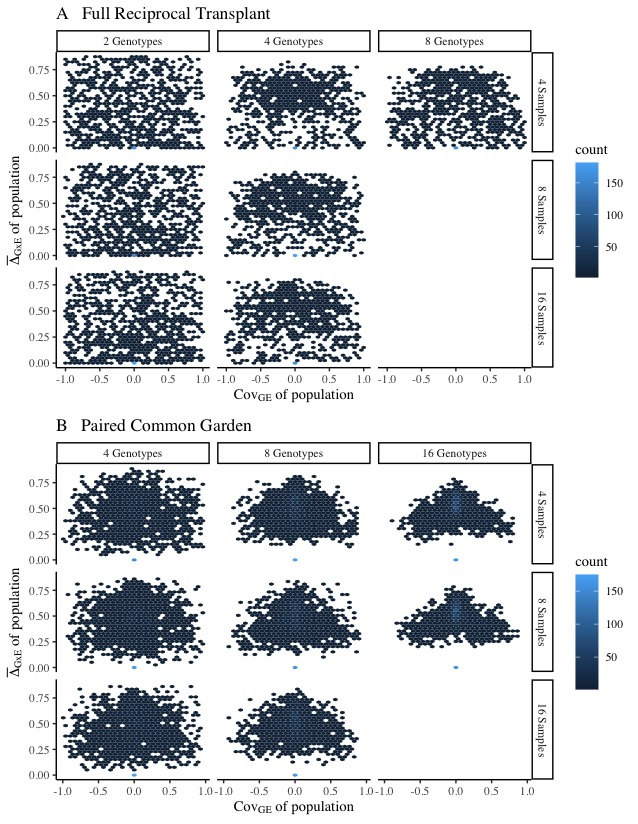
\includegraphics[width=6in]{3.11.HexPanel.jpeg}
\end{center}
\label{Fig: Parameter Coverage}
\caption{Coverage of parameter space of $Cov_{GE}$ and $\bar\Delta_{GxE}$ for full reciprocal transplant (A) and paired common garden designs (B). Hexagons are colored according to the density of observations in each bin. }
\end{figure}

\clearpage
\newpage

\renewcommand{\figurename}{Supplementary Figure}

\renewcommand\thefigure{S2}
\begin{figure}[h]
\begin{center}
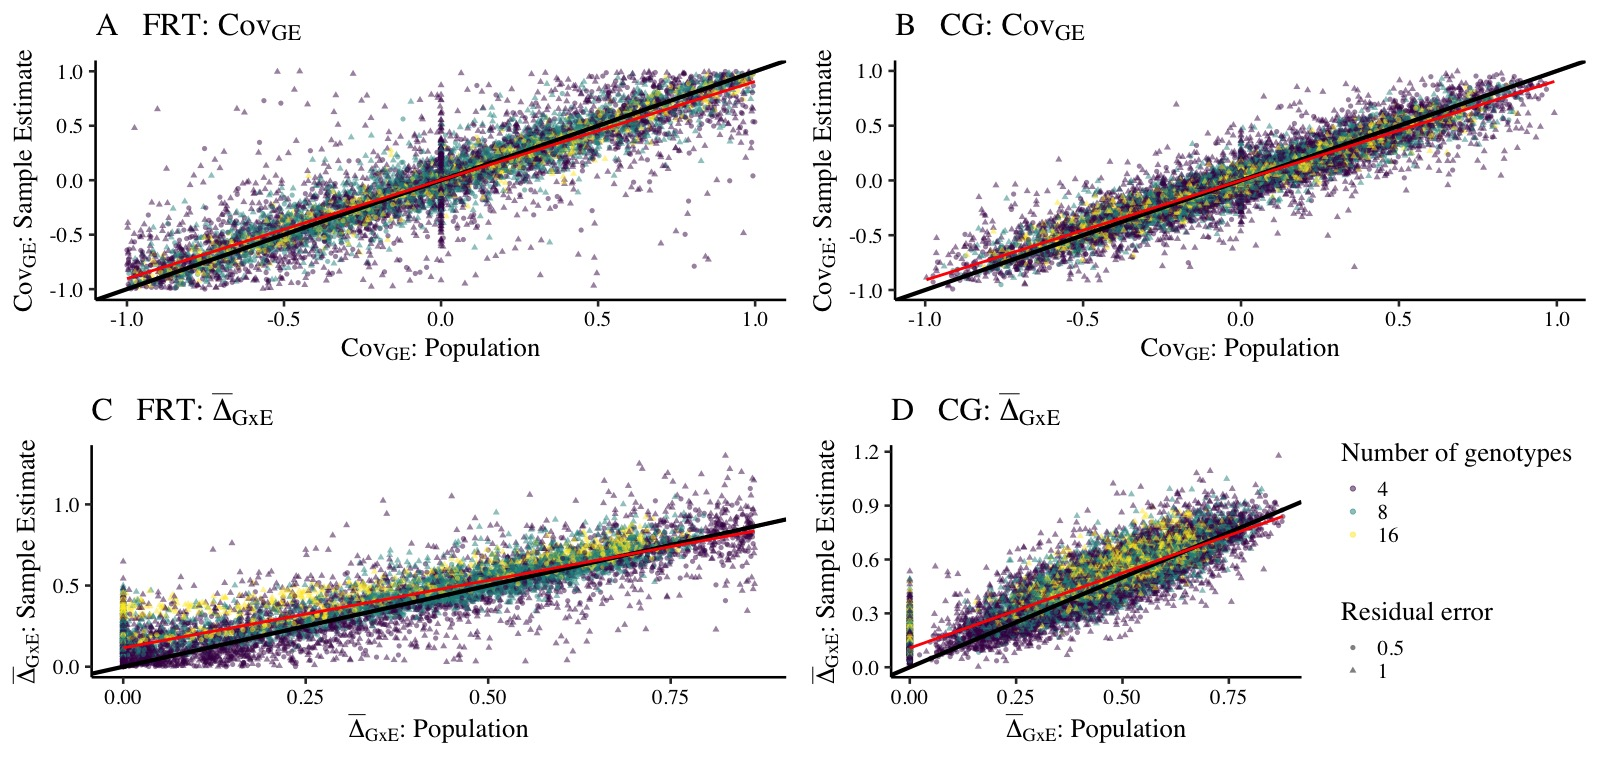
\includegraphics[width=6in]{3.11.SampleVsPopulation.jpeg}
\end{center}
\label{Fig: Population vs. Sample Estimates}
\caption{Agreement between population measures and sample estimates of $Cov_{GE}$ and $\bar\Delta_{GxE}$ for Full Reciprocal Transplant (A, C) and paired Common Garden designs (B, D). The black line falls along a 1:1 line while the red line reflects the pattern of the data. Point colors indicate the number of genotypes, while point shapes indicate the level of residual variation. As expected, sample estimates deviate more from the population measure in situations with low sample sizes and higher residual variation.}
\end{figure}

%\renewcommand{\figurename}{Supplementary Table}
%\renewcommand\thetable{S1}
%\begin{table}[]
%\begin{tabular}{lrrr}
%\hline
%Explanatory variable     & Estimate        & Standard Error   & z-value \\ \hline
%(Intercept)              & 27.95           & 6.67             & 4.19    \\
%Temperature              & -1.18           & 0.30             & -3.88   \\
%Copper Rockfish          & -20.58          & 6.78             & -3.04   \\
%Quillback Rockfish       & -24.01          & 6.71             & -3.58   \\
%Yellowtail Rockfish      & \textbf{112.06} & \textbf{5971.60} & 0.02    \\
%Temperature * Copper     & 0.91            & 0.31             & 2.94    \\
%Temperature * Quillback  & 1.00            & 0.31             & 3.27    \\
%Temperature * Yellowtail & -4.99           & 266.59           & -0.02   \\ \hline
%\end{tabular}
%\caption[Generalized linear model for mortality with Yellowtail coded as a Species.]{Results from the generalized linear model for mortality with Yellowtail coded as a Species. Note the coefficient inflation due to model overfitting (bold text).}
%\end{table}
%
%\clearpage
%\newpage
%
%%\renewcommand{\figurename}{Supplementary Figure}
%
%\renewcommand\thefigure{S1}
%\begin{figure}[h]
%\begin{center}
%\includegraphics[width=6in]{../S1-Mahalanobis.jpg}
%\end{center}
%\caption[Novel and disappearing climates in the global ocean.]{Novel and disappearing climates in the global ocean. Mahalanobis distance ($M_D$) represents the number of standard deviations a gridpoint differs from its closest analog in a global pool of data. The degree of disappearance is measured as the $M_D$ of a gridpoint from a timepoint in the past to a global pool of data from the future (left column, A, C, and E). The degree of novelty is measured as the $M_D$ of a gridpoint from a timepoint in the future to a global pool of data from the past (right column, B, D, and F).}
%\end{figure}
%
%
%\newpage
%\renewcommand\thefigure{S2}
%\begin{figure}[h]
%\begin{center}
%%\includegraphics[width=6in]{../S2.pdf}
%\end{center}
%\caption[Fig S2]{ 
%Blah blah 
%}
%\end{figure}
%
\end{document}